\documentclass{beamer}
%\mode<presentation> {
%\usetheme{metropolis}
%%\usefonttheme{professionalfonts}
\usepackage{fontspec}
\usepackage{listings}
\setsansfont{Futura}
%}
\usetheme{metropolis}
\metroset{
    titleformat=regular,
    sectionpage=progressbar,
    numbering=none,
    background=light,
}
\usepackage{appendixnumberbeamer}
\usepackage{setspace}
\usepackage{import}
\subimport{./shared/}{preamble.tex}
\subimport{./shared/}{project_definitions.tex}


\usetikzlibrary{overlay-beamer-styles}
\usepackage{booktabs}
\usepackage{caption}
\usepackage{csquotes}
\usepackage[scale=2]{ccicons}

%\usepackage{natbib}

\usepackage{pgfplots}
\usepgfplotslibrary{dateplot}

\usepackage{xspace}
\newcommand{\themename}{\textbf{\textsc{metropolis}}\xspace}

\usepackage{tikz} \tikzset{>=latex}
\usepackage{pgfplots,tikz}
\usepackage{amssymb}
\usepackage{empheq}
\usepackage{pdfpages}
\usepackage{mathtools}
\mathtoolsset{showonlyrefs}
\usepackage{amsmath}
\usepackage{esint}
\usepackage{multicol}
\usepackage{hyperref}
\usepackage{dirtytalk}
\usepackage{mdframed}
\usepackage{graphicx}
\graphicspath{ {images/} }

\newcommand{\fullPageImage}[1]{{
    \setbeamercolor{background canvas}{bg=black}
    \setbeamertemplate{navigation symbols}{}
    \begin{frame}[plain]
        \begin{tikzpicture}[remember picture,overlay]
            \node[at=(current page.center)] {
                \includegraphics[height=\paperheight]{#1}
            };
        \end{tikzpicture}
    \end{frame}
}}
\usetikzlibrary{decorations.markings}
\tikzstyle{vecArrow} = [thick, decoration={markings,mark=at position
   1 with {\arrow[semithick]{open triangle 60}}},
   double distance=1.4pt, shorten >= 5.5pt,
   preaction = {decorate},
   postaction = {draw,line width=1.4pt, white,shorten >= 4.5pt}]
\tikzstyle{innerWhite} = [semithick, white,line width=1.4pt, shorten >= 4.5pt]

%\usepackage{natbib}
\setbeamertemplate{frametitle continuation}[from second]
\renewcommand\bibfont{\scriptsize}

%\usepackage{rsc}
\renewcommand{\bibsection}{}

\newcommand{\newsection}[1]{
  %\metroset{background=dark}
    \section{#1}
  %\metroset{background=light}
}

%\newcommand{\theTitle}{An Interface for Future Comparison of Real and
%Simulated Interacting Galaxy Pair Morphologies using JSPAM}
%\newcommand{\theTitlecaps}{\MakeUppercase{\theTitle}}
%\newcommand{\theAuthor}{Jackson L. Cole}
%\newcommand{\theInstitution}{Middle Tennessee State University}

%%%%%%%%%%%%%%%%%%%%%%%%%%%%%%%%%%%%%%%%%%%%%%%%%%%%%%%%%%%%%%%%%%%%%%%%%%%%%%%%
\title[\theTitle]
{\theTitle}
\subtitle{}
\author{\theAuthor}
\institute[MTSU]
{
    \theInstitution\\
    \medskip
    \texttt{jlc2de@mtmail.mtsu.edu}\enspace\textbullet\enspace\texttt{jacksoncole.io}
}
\date{Fall 2018}

% for a full page image
%\fullPageImage{path/to/image.ext}
%%%%%%%%%%%%%%%%%%%%%%%%%%%%%%%%%%%%%%%%%%%%%%%%%%%%%%%%%%%%%%%%%%%%%%%%%%%%%%%%
\begin{document}
\begin{frame}
    \titlepage
\end{frame}

% --------------------------------------------------------------------------- %
%\newsection{Introduction}

\fullPageImage{./images/void.jpg}
\fullPageImage{./images/m51.jpg}

\begin{frame}%{Introduction}
    \begin{displayquote}
        It is double, each has a bright center, which are separated
        $4^{\prime}35^{\prime\prime}$.
        The two \say{atmospheres} touch each other, the one is even fainter than the
        other.\\
        {\hfill-Charles Messier \cite{Messier}}
    \end{displayquote}
\end{frame}

\begin{frame}{Importance of Collisions and Mergers}
    \begin{itemize}
        \item Galaxy mergers are important for large scale evolution of galaxies
            over the lifetime of the universe.
        \item Close encounters can increase the internal energies of galaxies on
            the same order of magnitude as their original internal
            energies. \cite{Alladin1965}
        \item Stars and other material can be flung into intergalactic space.
            \cite{Alladin1965}
    \end{itemize}
\end{frame}

\fullPageImage{./images/ant.jpg}

%\newsection{Background}

\begin{frame}{\citet{Toomre1972}}
    \begin{itemize}
        \item Prior to the early 1970s, many researchers opposed the idea that
            \say{bridges and tails} result from gravity alone
        \item Using \say{old-fashioned gravity}\dots
    \end{itemize}
\end{frame}

\fullPageImage{./images/toomre-paper.png}

\begin{frame}{JSPAM}
    \begin{itemize}
        \item Restricted three body code written in FORTRAN by Dr. John Wallin
            \cite{Wallin2016}
        \item Simulates mergers and produces data that can be used to
            render the resultant morphologies
    \end{itemize}
\end{frame}

\begin{frame}{Galaxy Zoo: Mergers \cite{holincheckThesis}}
    \begin{itemize}
        \item Citizen scientists volunteers were recruited to run the
            JSPAM software online and to determine \say{whether a simulation was
                'on the right track' or 'way off the mark'}
        \item At completion of project, over 3 million simulations had been
            reviewed.
        \item 66,395 sets of initial conditions that received Citizen Science
            score
    \end{itemize}
\end{frame}


\begin{frame}{Purpose}
    \begin{itemize}
        \item Provide a user-friendly interface to an inherently data-intensive
            project
        \item Provide a framework for producing data to be used in an
                image creation suite
        \item Provide tools that aid in creating an automatic image
        classification system using JSPAM
    \end{itemize}
\end{frame}

% --------------------------------------------------------------------------- %
\newsection{Methods}
% --------------------------------------------------------------------------- %
% --------------------------------------------------------------------------- %
\begin{frame}{Project Flowchart}
    \vspace{1em}
\begin{figure}[H]
    \centering

    \begin{tikzpicture}[thick, scale=0.5, every node/.style={scale=0.5}]
        \tikzstyle{every node}=[font=\scriptsize, style={scale=0.5}]
        \linespread{1}
        \node [startstop] (start)
        {START};

        \node [process, right = of start, text width=3cm](process_image)
        {Get, process image with MergerEx \cite{holincheckThesis}};

        \node [io, right = of process_image, yshift=1cm, text width=2cm] (mergerex_output_data)
        {OUTPUT: Merger data from MergerEx};

        \node [io, right = of process_image, yshift=-1cm, text width=2cm] (processed_image)
        {OUTPUT: SDSS DR7 image, processed};

        \node [process, right = of processed_image, text width=4cm] (used_in_comparisons)
        {Saved for comparison of simulation results with real images};

        \node [process, right = of mergerex_output_data, text width=4cm] (used_in_attributes)
        {Save as merger attributes in MergerRun instantiation};

        \node [io, below = of start.west, anchor=west, yshift=-1cm, text width=4cm] (inData1)
        {INPUT: target SDSSID, run number(s), n1\_particles, n2\_particles};

        \node [io, below = of inData1, text width=5cm] (inData2)
        {INPUT: Citizen Science initial conditions\\from run file for target SDSSID};

        \node [process, right = of inData2,] (JSPAM)
        {JSPAM (Wallincode)};

        \node [io, right = of JSPAM, text width=4cm] (outfile_root)
        {OUTPUT: Run data in root directory with distinguisher};

        \node [process, below = of inData2, text width=5cm] (directories)
        {Create appropriate directory structure};


        \node [process, below = of JSPAM, text width=5cm] (move_files)
        {Move output files to appropriate location in created directory structure};

        %\node [startstop, right = of move_files, text width=5cm] (stop)
        \node [startstop, below = of outfile_root] (stop)
        {STOP};


        \draw [arrow] (start) -- (process_image);
        \draw [arrow] (process_image) -| (mergerex_output_data);
        \draw [arrow] (mergerex_output_data) -- (used_in_attributes);
        \draw [arrow] (process_image) -| (processed_image);
        \draw [arrow] (processed_image) -- (used_in_comparisons);

        \draw [line] (used_in_comparisons.east) -- +(1,0);
        \draw [arrow] (used_in_attributes.east)  -- +(1,0) |- (inData1.east);
        \draw [arrow] (inData1) -- (inData2);
        \draw [arrow] (inData2) -- (JSPAM);
        \draw [arrow] (JSPAM) -- (outfile_root);
        \draw [arrow] (outfile_root) -- (directories);
        \draw [arrow] (directories) -- (move_files);
        \draw [arrow] (move_files) -- (stop);
        %\node [process, below = of JSPAM] (directories)
        %{Create appropriate directory structure};

        %\node [io, below = of directories, text width=12cm] (initialFile)
        %{
        %\{SDSSID\}.\{run number\}.i.\{n1\_particles\}.\{n2\_particles\}.txt\\
        %\{SDSSID\}.\{run number\}.f.\{n1\_particles\}.\{n2\_particles\}.txt\\
        %info.txt (from MergerEx \cite{holincheckThesis})
        %};

        %\node [process, below = of initialFile] (imageCreator)
        %{Create images};


        %\node [io, below = of imageCreator, text width = 2cm] (machineScore)
        %{Machine score};

        %\node [process, left = of machineScore] (comp)
        %{Comparison code};

        %\node [startstop, right = of machineScore] (stop)
        %{STOP};




    \end{tikzpicture}
    \caption{}
    %\caption[Project flowchart]{Flowchart describing how a run is processed and
    %    stored. It should be noted that tasks related to processing images with
    %    MergerEx must be done manually, but must only be done once. Further, the
    %    image creation suite that was developed alongside this project is not
    %    included here, as it is considered to be largely separate. It can be
    %    incorporated  immediately prior to \say{STOP}.
    %}
    \label{fig:flowchart}
\end{figure}
\end{frame}

\begin{frame}{Image Preparation and Target Data Acquisition}
    \begin{minipage}{0.5\linewidth}
    \begin{itemize}
        \item MergerEx \cite{Holincheck2015} for image acquisition and
            preparation
        \item Target data from MergerEx output
    \end{itemize}
    \end{minipage}%
    \begin{minipage}{0.5\linewidth}
        \begin{figure}[h]
            \centering
            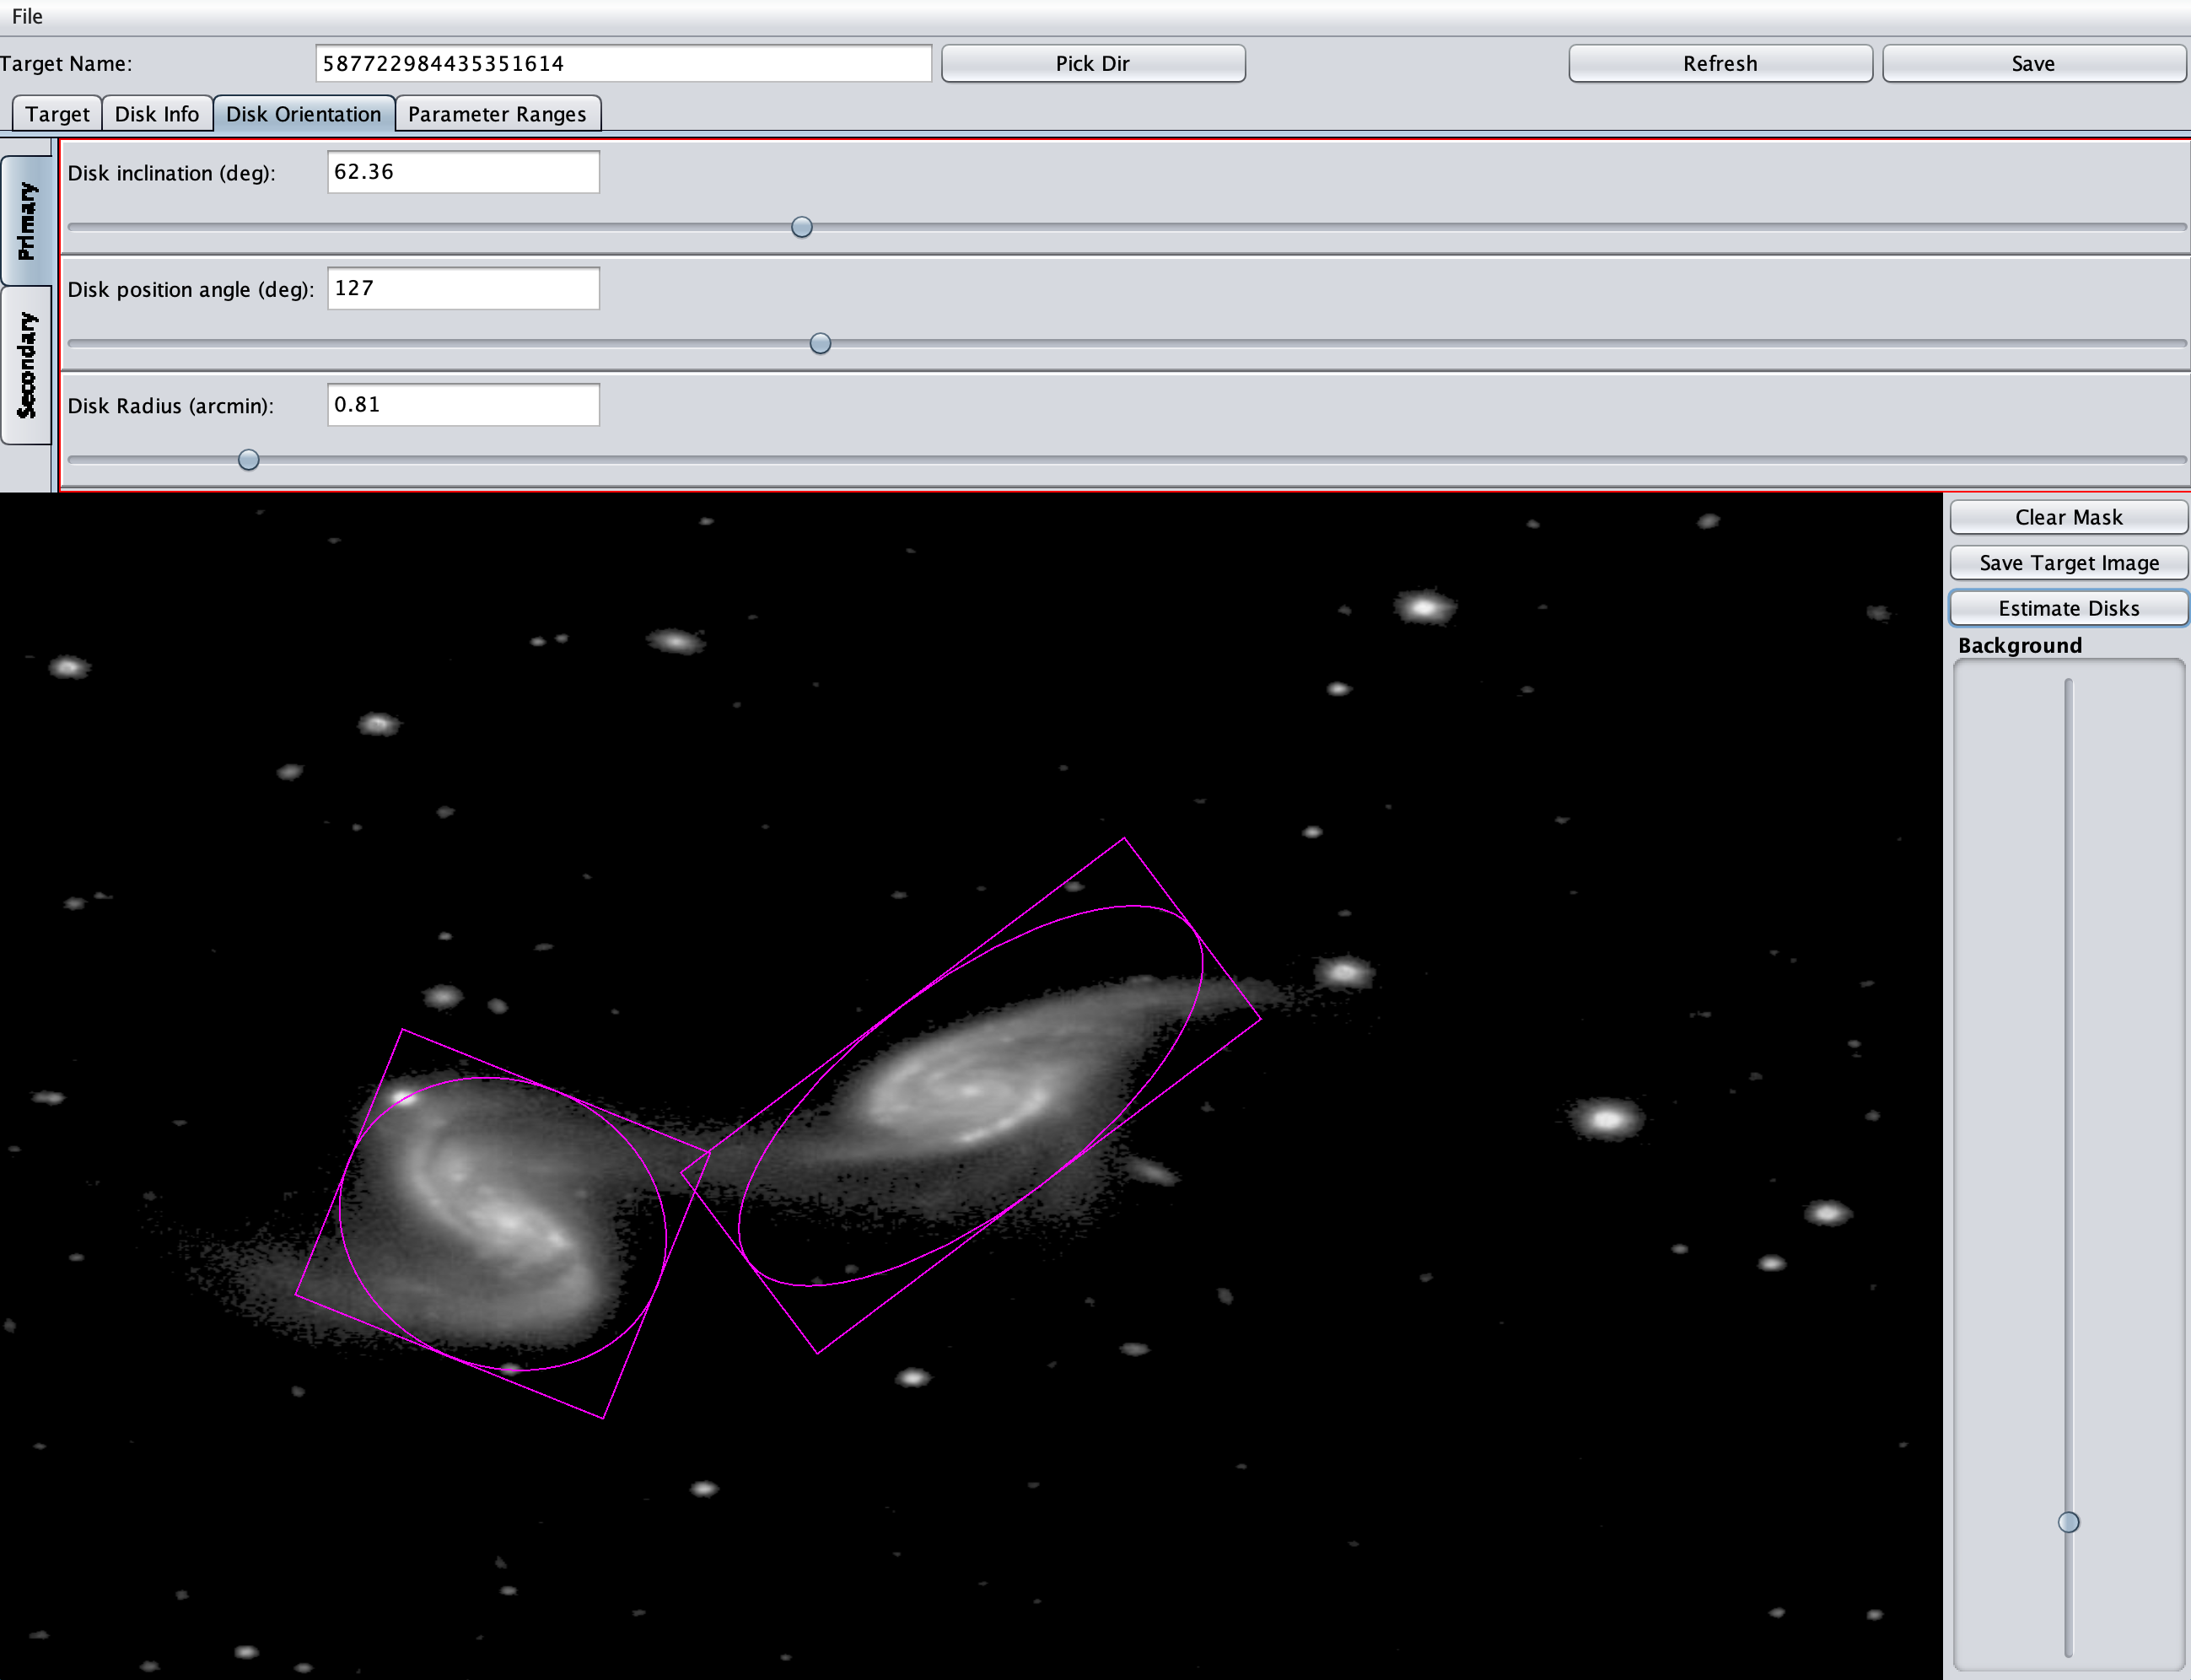
\includegraphics[width=0.9\linewidth]{./images/mergerex.png}
        \end{figure}
    \end{minipage}
\end{frame}

\begin{frame}[fragile]{Targets and Target Input Files}
    \begin{minipage}{0.5\textwidth}
    Targets:
    {\tiny\linespread{0.5}
    \dirtree{%
        .1 root.
        .2 targets.
        .3 \{SDSSID\}.
        .4 \{SDSSID\}.jpg.
        .4 \{SDSSID\}.calibrated.png.
        .4 \{SDSSID\}.info.txt.
        }
    }

    Target input files:
    {\tiny\linespread{0.5}
    \dirtree{%
        .1 root.
        .2 input.
        .3 \{SDSSID\}.txt.
        }
    }
    \end{minipage}%
    \begin{minipage}{0.5\textwidth}
        \begin{minipage}{0.5\linewidth}
        \begin{figure}[h]
            \centering
            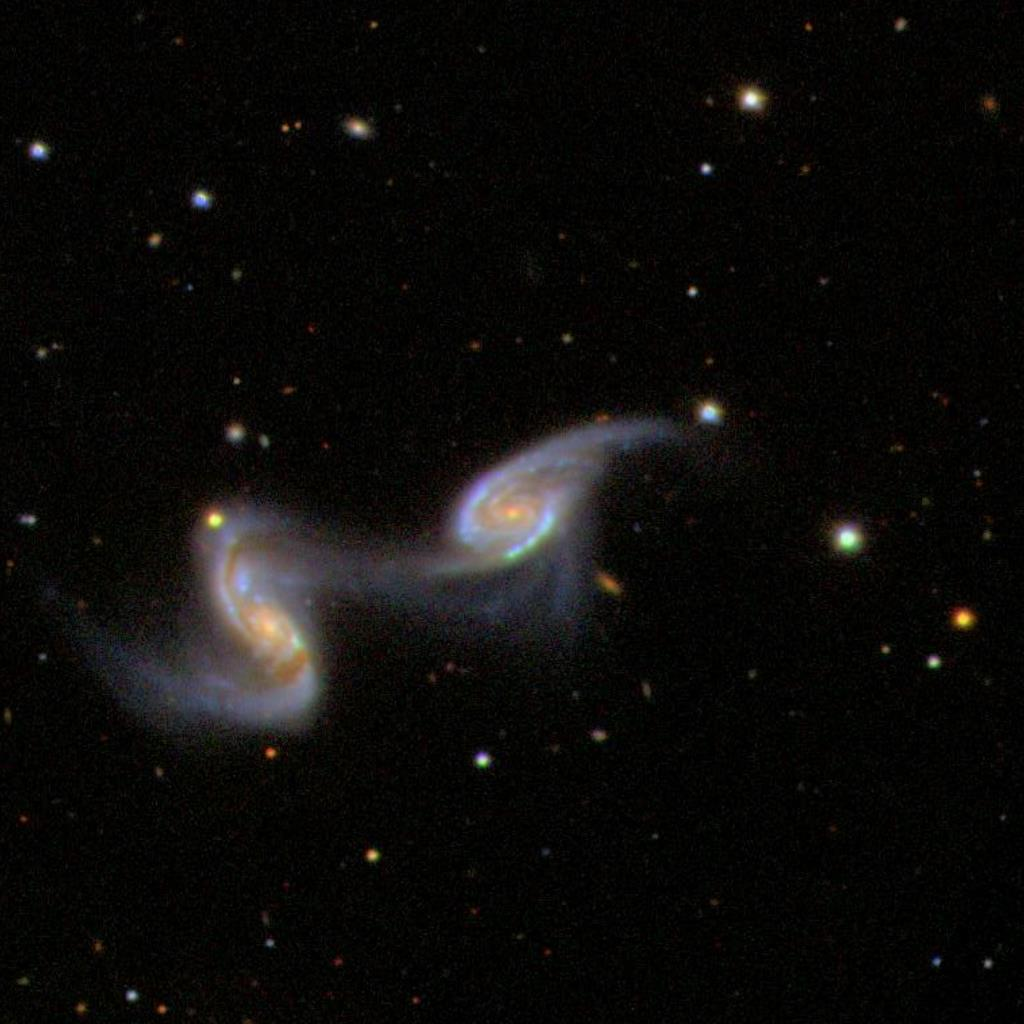
\includegraphics[width=0.95\linewidth]{./images/targets/generic/uncalibrated.png}
        \end{figure}%
        \end{minipage}%
        \begin{minipage}{0.5\linewidth}
        \begin{figure}[h]
            \centering
            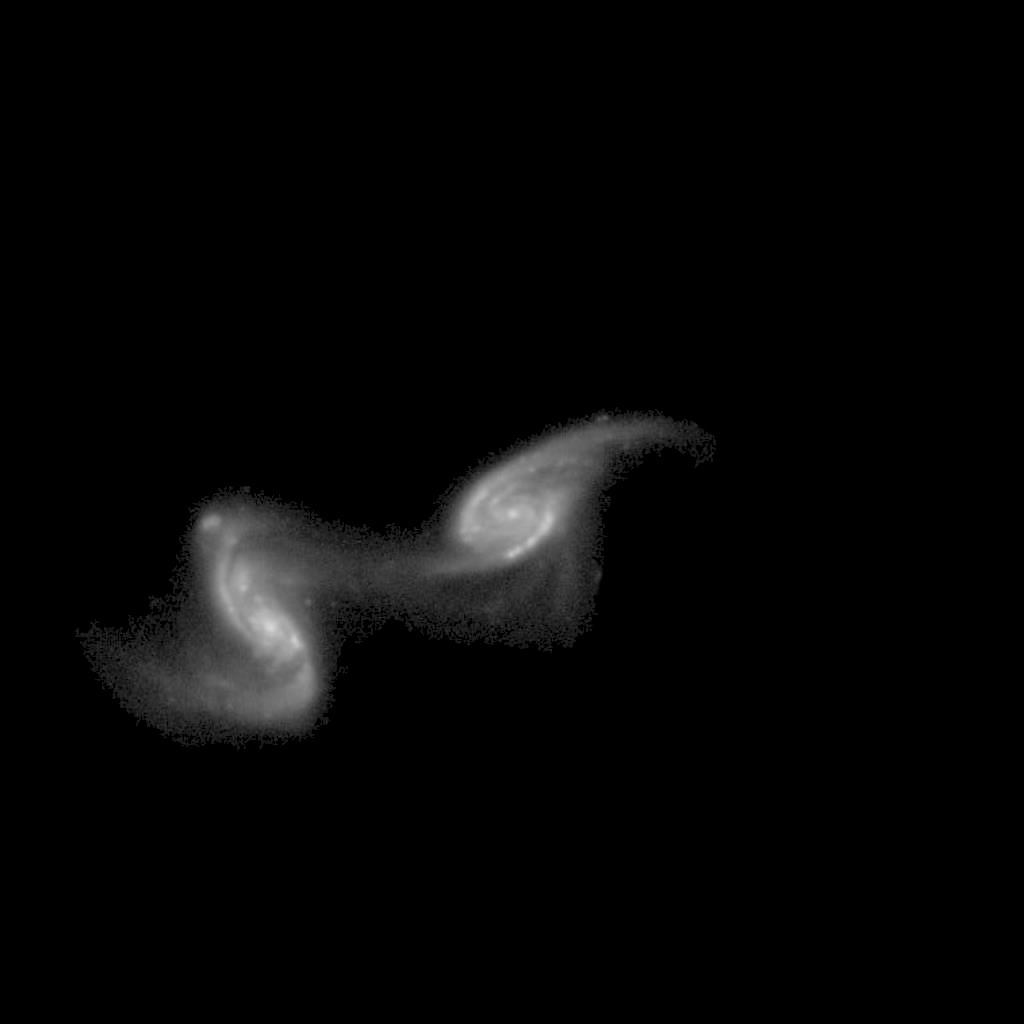
\includegraphics[width=0.95\linewidth]{./images/targets/generic/calibrated.png}
        \end{figure}
        \end{minipage}
        \lstset{basicstyle=\ttfamily\tiny,}
        \begin{lstlisting}
#target data file written Mon Mar 19 15:51:13 CDT 2018
name=587722984435351614
imagefile=587722984435351614.jpg
tgtimagefile=.tgt.png
imageheight=1024
imagewidth=1024
centerra=204.97048
centerdec=0.84004
imagesizearcmin=5.0

#primary disk info
pname=587722984435351614
.
.
.
\end{lstlisting}
    \end{minipage}
\end{frame}

\fullPageImage{./images/mergers-page.png}
\fullPageImage{./images/big-file.png}

\begin{frame}{Storage Methods}
    \begin{itemize}
        \item Explored the following options relating to data storage and
            retrieval:
            \begin{itemize}
                \item Databases
                \item Interfaces between FORTRAN, Python, and C++
                \item Binary data formats (HDF5)
                \item \alert{Flat files}
            \end{itemize}
    \end{itemize}
\end{frame}

\begin{frame}{Storage Structure and Naming Conventions}
%\begin{figure}[H]
    \scriptsize\linespread{0.5}
    \dirtree{%
        .1 root.
        .2 output.
        .3 \{SDSSID\}.
        .4 \{SDSSID\}.humanscores.txt.
        .4 run0000.
        .5 \{SDSSID\}.0000.i.\{n1\_particles\}.\{n2\_particles\}.txt.
        .5 \{SDSSID\}.0000.f.\{n1\_particles\}.\{n2\_particles\}.txt.
        .4 run0001.
        .5 \{SDSSID\}.0001.i.\{n1\_particles\}.\{n2\_particles\}.txt.
        .5 \{SDSSID\}.0001.f.\{n1\_particles\}.\{n2\_particles\}.txt.
        %.4 run0002.
        %.5 \{SDSSID\}.0002.i.\{n1\_particles\}.\{n2\_particles\}.txt.
        %.5 \{SDSSID\}.0002.f.\{n1\_particles\}.\{n2\_particles\}.txt.
        .4 run\ldots.
        .5 \{SDSSID\}.\{\ldots\}.i.\{n1\_particles\}.\{n2\_particles\}.txt.
        .5 \{SDSSID\}.\{\ldots\}.f.\{n1\_particles\}.\{n2\_particles\}.txt.
    }
%    \caption[Output directory tree]{Output directory tree}
%    \label{fig:the_tree}
%\end{figure}
\end{frame}




%\begin{frame}{Galaxy Class}
%    \subimport{./content/methods/uml/}{galaxy.tex}
%\end{frame}

%\begin{frame}{\texttt{MergerRun}}
%\begin{figure}[H]
%    \centering
%    \begin{tikzpicture}[scale=0.6, every node/.style={scale=0.6}]
%        \linespread{1}
%        \begin{class}[font=\ttfamily\footnotesize, text width=12cm]{MergerRun}{0,0}
%            \attribute{info : dictionary}
%            \attribute{name : string}
%            \attribute{height : Size instance}
%            \attribute{width : Size instance}
%            \attribute{dimensions : Dimensions instance}
%            \attribute{filename : string}
%            \attribute{humanscores\_filename : string}
%            \attribute{run : integer}
%            \attribute{init : string}
%            \attribute{structure\_created : boolean}
%            \attribute{target\_dirs : string(path/to/target\_directory)}
%            \attribute{primary : Galaxy instance}
%            \attribute{secondary : Galaxy instance}
%            \attribute{all\_point\_data : list}
%            \attribute{scores : list}
%            \operation[0]{\_\_init\_\_(path\_to\_info\_file, n1\_particles, n2\_particles, run\_number, init\_run\_string) : MergerRun instance}
%            \operation[0]{make\_info\_dict(path\_to\_info\_file) : dictionary}
%            \operation[0]{setup\_structure(path\_to\_info\_file) : dictionary}
%            \operation[0]{existing\_structure()}
%            \operation[0]{create()}
%            \operation[0]{get\_scores()}
%            \operation[0]{write\_scores()}
%            \operation[0]{load\_data() : list}
%            \operation[0]{fill\_all\_data() : list}
%            \operation[0]{plotting\_2d() : figure}
%            \operation[0]{plotting\_3d() : figure}
%            \operation[0]{make\_gif()}
%        \end{class}
%    \end{tikzpicture}
%    \caption[Class diagram: MergerRun]{Class diagram: MergerRun}
%    \label{fig:cdmergerrun}
%\end{figure}
%\end{frame}

\begin{frame}{JSPAM Command Line Interface}
    \begin{itemize}
        \item Standardizes interaction with JSPAM
        \item Handles all data retrieval and storage
        \item Provides objects for encapsulating all data related to merger runs
        \item Begins push toward removing the human-in-the-loop
    \end{itemize}
\end{frame}

\begin{frame}{\texttt{jspamcli.py} Usage}
    %\myworries{The table below needs to be centered}
    \centering
    \begin{figure}
\begin{table}[h!]
    \scriptsize
    %\centering
    \begin{tabular}{clll}
    \toprule
    Mode & Option       & Behavior                        & Arguments \\
    \midrule
    $1$ & \texttt{-i}  & run interactively               & NONE          \\
    $2$ & \texttt{-bi} & batch process interactively     & NONE          \\
    $3$ & \texttt{-b}  & batch process (normal)%
        & \texttt{batch\_run\_file}\ldots\\
    $4$ & \texttt{-bm} & batch processing on multiple cores & \texttt{num\_cores}
    \texttt{batch\_run\_file}\\
    $5$ & \texttt{-g}  & GIF Creation Tool               & NONE          \\
    \bottomrule
    \end{tabular}
    \caption[\texttt{jspamcli.py} command line options]%
    {List of command line options
        available in \texttt{jspamcli.py}. In the \texttt{-b} and \texttt{-bm}
        modes, multiple batch run files may be specified as long as they exist in
        the \texttt{batch\_run\_files} directory in the root directory.
    }
    \label{table:jspamcli_table}
\end{table}
\end{figure}
\end{frame}

\begin{frame}{GIF Creation Tool}
    \url{https://github.com/jacksonlanecole/WallinCode-restructure/blob/master/docs/example.mp4}
\end{frame}

\begin{frame}{Comparison of Methods in Running All Possible Simulations}
    \vspace{1em}
\begin{figure}[H]
    \centering
    \begin{minipage}{0.5\textwidth}
    \begin{tikzpicture}[thick, scale=0.5, every node/.style={scale=0.5}]
        \tikzstyle{every node}=[node distance=1em, font=\small, style={scale=0.5}]
        \linespread{1}
        \node [startstop] (start)
        {START};

        \node [process, below = of start, text width=5cm](determine_runs)
        {Determine target, run/runs, parameters for each run};

        \node [process, below = of determine_runs, text width=5cm](dl_data)
        {Download and unzip target data};

        \node [process, below = of dl_data, text width=8cm](cpandpaste)
        {Copy parameter string corresponding to run};

        \node [process, below = of cpandpaste, text width=10cm](basic_run)
        {\texttt{basic\_run -m 1 -n1 5000 -n2 5000 (paste parameter string)}};

        \node[process, below = of basic_run, text width=5cm](organize_output)
        {Organize, rename output files};

        \node[startstop, below = of organize_output] (stop)
        {STOP};

        \draw[arrow] (start) -- (determine_runs);
        \draw[arrow] (determine_runs) -- (dl_data);
        \draw[arrow] (dl_data) -- (cpandpaste);
        \draw[arrow] (cpandpaste) -- (basic_run);
        \draw[arrow] (basic_run) -- (organize_output);
        \draw[arrow] (organize_output) -- (stop);

    \end{tikzpicture}
    \begin{center}
        \alert{>66000 times}
    \end{center}
    \end{minipage}%
    \begin{minipage}{0.5\textwidth}
    \begin{tikzpicture}[thick, scale=0.5, every node/.style={scale=0.5}]
        \tikzstyle{every node}=[node distance=2em, font=\small, style={scale=0.5}]
        \linespread{1}
        \node [startstop] (start)
        {START};

        \node [process, below = of start, text width=5cm](determine_runs)
        {Determine target, run/runs, parameters for each run};

        \node [process, below = of determine_runs, text width=10cm](jspamcli)
        {\texttt{python jspamcli.py [options] [batch run file names \dots]}};


        \node[startstop, below = of jspamcli] (stop)
        {STOP};

        \draw[arrow] (start) -- (determine_runs);
        \draw[arrow] (determine_runs) -- (jspamcli);
        \draw[arrow] (jspamcli) -- (stop);

    \end{tikzpicture}
    \end{minipage}
\end{figure}

\end{frame}



%\newsection{Results and Conclusions}
\begin{frame}{Results and Conclusions}
    Overall
    \begin{itemize}
        \item This work takes care of tasks that are standard in any
            future work using the JSPAM software.
        \item New users beginning work on projects using JSPAM should be able to
            use/augment our code for their purposes
    \end{itemize}

    Personal
    \begin{itemize}
        \item Became much more comfortable writing, maintaining, documenting
            Python code efficiently
        \item Improved my usage of version control tools to keep track of all
            changes made to existing code
    \end{itemize}
\end{frame}

\begin{frame}[t,allowframebreaks]
    \frametitle{References}
    \bibliography{thesisbib}
\end{frame}

\end{document}
